% template from https://fachschaft.tf.uni-freiburg.de/informationen/dokumentvorlagen
%
%
%
% documentclass options:
\documentclass[11pt,
  a4paper,
  parskip=half, % This is some extra vertical space between paragraphs, the suggestion is 2cm which is really ugly, so we use what koma script gives us
  % you can also set it to full for even more space. But there is a bad tex style decision: parskip also changes the spacing between listitems such as
  % enumerate and itemize. For this purpose we include the enumitem package and set itemsep=.5em, of course you can change this
  BCOR=10mm, % BCOR is binding correction
  ngerman,
  % if you'd rather have a one sided thesis, add `oneside' to the documentclass
  % onside,
  % ngerman is needed for hyphenation if the thesis contains parts written in German, switch order with english if you write mainly in English.
  % Remember to change order in the babel package (below) as well.
  % Last language is the preferred one.
  english]{scrbook}
\usepackage[ngerman,english]{babel} % If you write mainly in English change order to ngerman, english. Also change that in the documentclass options above.
% Include of titling must happen before \title etc.
% that's why it's not in setup.tex
\usepackage{titling}
\title{Semantic approaches to citation recommendation}
\author{Tarek Saier}

% Change to your first examiner
% The ~ enables non sentence spacing after a period
\newcommand{\firstexaminer}{Prof.~Dr.~Georg Lausen}
% Change to your second examiner, some undergraduate studies don't have a second examiner
% in this case just comment out the following line
\newcommand{\secondexaminer}{Dr.~Michael F{\"{a}}rber}
% Change to your adivers
\newcommand{\advisers}{Dr.~Michael F{\"{a}}rber}

% include all packages and define commands in setup.tex

%------------------------------------------------------------------------------
%       package includes
%------------------------------------------------------------------------------
    % font encoding is set up for pdflatex, for other environments see
    % http://tex.stackexchange.com/questions/44694/fontenc-vs-inputenc
    \usepackage[T1]{fontenc}  % 8-bit fonts, improves handling of hyphenations
    \usepackage[utf8]{inputenc}  % remove if engine is switched to xelatex
    % provides `old' commands for table of contents. Eases the ability to switch
    % between book and scrbook
    \usepackage{scrhack}

    % better looking fonts
    \usepackage[tt=false, type1=true]{libertine}
    \usepackage{libertinust1math}


    % ------------------- layout, default -------------------
    % adjust the style of float's captions, separated from text to improve readabilty
    \usepackage[labelfont=bf, labelsep=colon, format=hang, textfont=singlespacing]{caption}
    % With format = hang your caption will look like this:
    % Figure 1: Lorem ipsum dolor sit amet,
    %           consectetuer adipiscing elit.
    %           Ut purus elit, vestibulum
    % If you instead want
    % Figure 1: Lorem ipsum dolor sit amet,
    % consectetuer adipiscing elit. Ut purus
    % elit, vestibulum
    % change to format=plain
    \usepackage{chngcntr}  % continuous numbering of figures/tables over chapters
    \counterwithout{equation}{chapter}
    \counterwithout{figure}{chapter}
    \counterwithout{table}{chapter}

    % Uncomment the following line if you switch from scrbook to book
    % and comment the setkomafont line
    %\usepackage{titlesec}  % remove "Chapter" from the chapter title
    %\titleformat{\chapter}[hang]{\bfseries\huge}{\thechapter}{2pc}{\huge}
    \setkomafont{chapter}{\normalfont\bfseries\huge}

    \usepackage{setspace}  % Line spacing
    \onehalfspacing
    % \doublespacing  % uncomment for double spacing, e.g. for annotations in correction

    % ------------------- functional, default-------------------
    \usepackage[dvipsnames]{xcolor}  % more colors
    \usepackage{array}  % custom format per column in table - needed on the title page
    \usepackage{graphicx}  % include graphics
    \usepackage{subfig}  % divide figure, e.g. 1(a), 1(b)...
    \usepackage{amsmath}  % |
    \usepackage{amsthm}   % | math, bmatrix etc
    \usepackage{amsfonts} % |
    \usepackage{calc}  % calculate within LaTeX
    \usepackage[unicode=true,bookmarks=true,bookmarksnumbered=true,
                bookmarksopen=true,bookmarksopenlevel=1,breaklinks=false,
                pdfborder={0 0 0},backref=false,colorlinks=false]{hyperref}
    \usepackage{etoolbox} % if-else commands


    %==========================================
    % You might not need the following packages, I only included them as they
    % are needed for the example floats
    % ------------------- functional, custom -------------------
    \usepackage{algorithm,algpseudocode}
    \usepackage{bm}  % bold greek variables (boldmath)
    % \usepackage{tikz}
    % \usetikzlibrary{positioning}  % use: above left of, etc

    % Improves general appearance of the text
    \usepackage[protrusion=true,expansion=true, kerning]{microtype}
    % \usepackage[protrusion=true]{microtype} % in case a switch to xelatex is
    %                                           necessary
    \usepackage{enumitem}

    % usually you don't need this, just for demonstration of a longer caption
    % \usepackage{lipsum}

    % toprule/midrule style tables
    \usepackage{booktabs}
    % make footnotes in tables work
    \usepackage{footnote}
    \makesavenoteenv{tabular}
    \makesavenoteenv{table}
    % enable listings
    \usepackage{listings}
    \lstset{literate=
      {Ş}{{\c{S}}}1 {ğ}{{\v{g}}}1,
      frame=top,frame=bottom,
      breaklines=true,
      basicstyle=\linespread{1}\footnotesize\ttfamily,
      escapeinside={(*}{*)}
    }

%------------------------------------------------------------------------------
%       (re)new commands / settings
%------------------------------------------------------------------------------
    % ----------------- referencing ----------------
    \newcommand{\secref}[1]{Section~\ref{#1}}
    \newcommand{\chapref}[1]{Chapter~\ref{#1}}
    \renewcommand{\eqref}[1]{Equation~(\ref{#1})}
    \newcommand{\figref}[1]{Figure~\ref{#1}}
    \newcommand{\tabref}[1]{Table~\ref{#1}}

    % ------------------- colors -------------------
    \definecolor{darkgreen}{rgb}{0.0, 0.5, 0.0}
    % Colors of the Albert Ludwigs University as in
    % https://www.zuv.uni-freiburg.de/service/cd/cd-manual/farbwelt
    \definecolor{UniBlue}{RGB}{0, 74, 153}
    \definecolor{UniRed}{RGB}{193, 0, 42}
    \definecolor{UniGrey}{RGB}{154, 155, 156}


    % ------------------- layout -------------------
    % prevents floating objects from being placed ahead of their section
    \let\mySection\section\renewcommand{\section}{\suppressfloats[t]\mySection}
    \let\mySubSection\subsection\renewcommand{\subsection}{\suppressfloats[t]\mySubSection}


    % ------------------- marker commands -------------------
    % ToDo command
    \newcommand{\todo}[1]{\textbf{\textcolor{red}{(TODO: #1)}}}
    \newcommand{\extend}[1]{\textbf{\textcolor{darkgreen}{(EXTEND: #1)}}}
    % Lighter color to note down quick drafts
    \newcommand{\draft}[1]{\textbf{\textcolor{NavyBlue}{(DRAFT: #1)}}}


    % ------------------- math formatting commands -------------------
    % define vectors to be bold instead of using an arrow
    \renewcommand{\vec}[1]{\mathbf{#1}}
    \newcommand{\mat}[1]{\mathbf{#1}}
    % tag equation with name
    \newcommand{\eqname}[1]{\tag*{#1}}


    % ------------------- pdf settings -------------------
    % ADAPT THIS
    \hypersetup{pdftitle={\thetitle},
                pdfauthor={\theauthor},
                pdfsubject={Master's thesis at the Albert Ludwig University of Freiburg},
                pdfkeywords={citation recommendation, recommender system, data set, master thesis},
                pdfpagelayout=OneColumn, pdfnewwindow=true, pdfstartview=XYZ, plainpages=false}


    %==========================================
    % You might not need the following commands, I only included them as they
    % are needed for the example floats

    % ------------------- Tikz styles -------------------
    % \tikzset{>=latex}  % arrow style

    % ------------------- algorithm ---------------------
    % Command to align comments in algorithm
    \newcommand{\alignedComment}[1]{\Comment{\parbox[t]{.35\linewidth}{#1}}}
    % define a foreach command in algorithms
    \algnewcommand\algorithmicforeach{\textbf{foreach}}
    \algdef{S}[FOR]{ForEach}[1]{\algorithmicforeach\ #1\ \algorithmicdo}

    % line spacing should be 1.5
    \renewcommand{\baselinestretch}{1.5}

    % set distance between items in a list, for more details see the
    % enumitem package: https://www.ctan.org/pkg/enumitem
    \setlist{topsep=0pt,itemsep=0ex,partopsep=1ex,parsep=0ex}


\begin{document}
    \pagestyle{empty} % no header and no page number
    % disable hyper links to remove warning "destination with same identifier"
    % this means within this section nothing can be referenced with a hyperlink
    \hypersetup{pageanchor=false}

    % enable/disable, depending on your chosen language
    
\begin{titlepage}
\begin{center}

\newcommand{\HorizontalLine}{\rule{\linewidth}{0.3mm}}

{\Large Master's Thesis}\\[1.3cm]


% _____________________________________________________________________________
\HorizontalLine \\[0.4cm]
% Write your title in a fancy way like this if you want to customize it, otherwise simply let tex do it for you
% \begin{spacing}{3}
%     {\huge \bfseries The Long, Long } \\
%     {\huge \bfseries Long Long} \\
%     {\huge \bfseries Title}\\
% \end{spacing}
{ \huge \bfseries \thetitle }
\HorizontalLine \\[1.5cm]
% _____________________________________________________________________________


{\Huge \theauthor} \\[2cm]


\begin{tabular}[hc]{>{\huge}l >{\huge}l}
  Examiners: & \firstexaminer \\[0.3cm]
             & \secondexaminer \\[1.2cm]
\end{tabular}
\vfill  % move the following text to the bottom

\Large {
    Albert-Ludwigs-University Freiburg\\
    Faculty of Engineering\\
    Department of Computer Science\\
    Chair of Databases and Information Systems\\[1cm]

    April 30\textsuperscript{th}, 2019\\
}
\end{center}
\end{titlepage}

\thispagestyle{empty}
% title page back
\ \vfill \ \\  % at least one space required before vfill
\
\textbf{Writing Period}            \smallskip{} \\
15.\,10.\,2018 -- 30.\,04.\,2019   \bigskip{} \\
\
\textbf{First Examiner}                  \smallskip{} \\
\firstexaminer                     \bigskip{} \\
\
% If there is a second examiner include it
\ifdef{\secondexaminer}
	{
	% Include
	\textbf{Second Examiner \& Supervisor}       \smallskip{} \\
	\secondexaminer                \bigskip{} \\
	\
	}
	{
	% No second examiner, ignore
	}
% \textbf{Supervisor}                  \smallskip{} \\
% \advisers

    \begin{titlepage}
\begin{center}

\newcommand{\HorizontalLine}{\rule{\linewidth}{0.3mm}}

{\Large Master-Thesis}\\[1.3cm]


% _____________________________________________________________________________
\HorizontalLine \\[0.4cm]
% Write yourtitle in a fancy way like this if you want to customize it, otherwise simply let tex do it for you
% \begin{spacing}{3}
%     {\huge \bfseries Der Lange, Lange } \\
%     {\huge \bfseries Lange Lange} \\
%     {\huge \bfseries Titel}\\
% \end{spacing}
{ \huge \bfseries \thetitle }
\HorizontalLine \\[1.5cm]
% _____________________________________________________________________________


{\Huge \theauthor} \\[2cm]


\begin{tabular}[hc]{>{\huge}l >{\huge}l}
  Gutachter: & \firstexaminer \\[0.3cm]
             & \secondexaminer \\[1.2cm]
\end{tabular}
\vfill  % move the following text to the bottom

\Large {
    Albert-Ludwigs-Universität Freiburg\\
    Technische Fakultät\\
    Institut für Informatik\\
    Lehrstuhl für Datenbanken und Informationssysteme\\[1cm]

    30. April 2019
    \\
}
\end{center}
\end{titlepage}

\thispagestyle{empty}
% title page back
\ \vfill \ \\  % at least one space required before vfill
\
\textbf{Bearbeitungszeit}            \smallskip{} \\
15.\,10.\,2018 -- 30.\,04.\,2019   \bigskip{} \\
\
\textbf{Erstgutachter}                  \smallskip{} \\
\firstexaminer                      \bigskip{} \\
\
% If there is a second examiner include it
\ifdef{\secondexaminer}
	{
	% Include
	\textbf{Zweitgutachter \& Betreuer}        \smallskip{} \\
	\secondexaminer                \bigskip{} \\
	\
	}
	{
	% No second examiner, ignore
	}
% \textbf{Betreuer}                  \smallskip{} \\
% \advisers


    \pagestyle{plain} % remove chapter name from top, page number at the bottom
    % use \pagestyle{headings} for having the chapter on top of the pages
    % if you want a more fancy header use \usepackage[automark,headsepline]{scrlayer-scrpage}
    % and read about it in the KOMA script documentation, https://www.ctan.org/pkg/koma-script
    \frontmatter  % roman page numbers
    % official declaration from the examination office
% copied from https://www.tf.uni-freiburg.de/de/studium-lehre/a-bis-z-studium/dokumente/Declarationforthefinalthesis.pdf

\chapter*{Declaration}

I hereby declare, that I am the sole author and composer of my thesis and that no other sources or learning aids, other than those listed, have been used. Furthermore, I declare that I have acknowledged the work of others by providing detailed references of said work.  \newline
I also hereby declare, that my thesis has not been prepared for another examination
or assignment, either in its entirety or excerpts thereof.
\\[3\normalbaselineskip]
\begin{tabular}{p{\textwidth/2} l}
  \rule{\textwidth/3}{0.4pt}   &   \rule{\textwidth/3}{0.4pt} \\
  Place, Date                  &   Signature
\end{tabular}

    \chapter*{Abstract}
New research is being published at a rate, at which it is %
%practically
infeasible for many scholars, to read and assess everything possibly %
%/that could possibly be
relevant to their work. %
In pursuit of a remedy, efforts towards automated processing of publications, like semantic modelling of papers to facilitate their digital handling, and the development of information filtering systems, are an active area of research. %
% maybe add a sentence here, leading from research in this
% area *in general* to citation recommendation
In this thesis, we investigate the semantic modelling of citation contexts for the purpose of citation recommendation. For this, we generate a large data set with accurate citation information from publications' \LaTeX{} sources on arXiv.org. Using this data set, we develop recommendation models based on entities and claim structures. To assess the effectiveness and conceptual soundness of our models, we perform a large offline evaluation on our own as well as several established data sets and furthermore conduct a user study. Our findings show that the models can outperform a non-semantic baseline model and do, indeed, capture the kind of information they're conceptualized for.
%In evaluating our models on several data sets and through a user study, we show that they can outperform a non-semantic baseline and are especially well suited for the recommendation of the types of citations they're conceptualized for.

%Citation recommendation systems, a possible remedy, 
%Researchers spent a considerable amount of time identifying publications that are worthwhile reading and appropriate to reference. The development of systems to aid in these tasks is an active area of research.
%Citations are the means by which scholars relate their research to existing work, 

\chapter*{Zusammenfassung}
fu bar

    \tableofcontents
    \listoffigures
    \listoftables
    \listofalgorithms
    \hypersetup{pageanchor=true}  % re-enable hyperlinking

    \mainmatter  % Arabic page numbers
    \chapter{Introduction}\label{chap:introduction}
\section{Motivation}
Citations are a central building block of scholarly discourse. They are the means by which scholars relate their research to existing work---be it in backing up claims, criticising, naming examples or engaging in any other form. Citing in a meaningful way requires an author to be aware of publications relevant to their work.
Here, the ever increasing amount of new reseach publications per year poses a serious challenge. Even with academic search engines like Goolge Scholar and CiteSeer$^X$ at our disposal, identifying publications that are worthwhile to examine and appropriate to reference remains a time consuming task.

It is therefore not suprising that methods to aid researchers in these tasks have been and still are being actively researched. While diverse in nature, the common core of these efforts is the goal to utilize the automated processing of publications. This can be achieved by either extracting information from publications as they are~\cite{Nasar2018,Beel2016}, or by introducing explicit semantic representations of their content or interrelations to facilitate automated processing~\cite{BuckinghamShum2000,Schneider2013,Jaradeh2019}. % TODO: mby distinguish between metadata and annotation/representation of content here (for the latter mby name JATS)
Once processed, a typical method is to harvest human made citations, analyze them~\cite{Abujbara2013,Teufel2006a} and use them for example to recommend papers~\cite{Beel2016} or aid in document exploration~\cite{Berger2016}. Although systems like this have existed for over 20 years~\cite{Bollacker1998,Beel2016}, there is not a lot of work looking into the use of explicit semantic representations for the recommendation of papers.
% ,Kitamoto2015 (after BuckinghamShum and Schneider)
% TODO: mby add sth about what the prospective benefits of semantic representations would be (e.g. if rather advanced model: search for citations for certain claims instead of just keyword based)
This is why this thesis will investiage their application. More specifically, we will concentrate on the task of recommending papers for citation---as opposed to, for example, discovery. What this encompasses will be described in more detail in the following section.

%Teufel2006b

% Systems for recommending papers have existed since 1998~\cite{Bollacker1998,Beel2016}. The closely related field of citation analysis has an even longer history that spans multiple disciplices including applied linguistics, history and sociology of sience and information science~\cite{Swales1986,White2004}.

% also there’s different approaches to it (collab.fil. / content based fil.(input=paper / input=sentence / input=sentence+one citation\cite{Kobayashi2018} / input=abstract\cite{Ayala-Gomez2018}) / graph based)

\section{Problem setting}\label{sec:problemsetting}
In the boradest sense, recommending papers for citation means given an input text, suggest publications that can be referred to from within that text. In scale this can vary from specific recommendations for a section of a sentence (\emph{local} or \emph{context-based}), to general recommendations for a whole input document (\emph{global}). The task can also include deciding whether or not the input contains parts that would justify inserting a citation in the first place~\cite{He2011}. In this thesis, we will focus on local citation recommendation with the assumption that the input always allows for/requires a citation to be put in.

Another distinction to be made is between personalized and general citation recommendation. Some approaches make use of user specific information such as an author's prior citations. Collaborative filtering approaches by nature include a user model and therfore fall into this category. While personalization can improve recommendation, it limits the approach to users that are willing to share personal information. % also if prior own publications would be needed (to see what authors, venues, fields of study one cites) there would be an interesting version of the could start problem. worth mentioning?
We therefore limit ourselves to purely content based filtering approaches.
% TODO: add argument for only using contexts to describe cited docs and not also title, abstract, metadata (mby cite \cite{Elkiss2008}) (possible argument: first only investigate semantic representations of citation contexts, then (future work) look into combining this information with other data)

A last clarification has to be made concerning the term \emph{explicit semantic representations}. This is to be understood as a differentiation from the mere use of unstructured text. A most prominent example for explicit semantic representations would be the structure of the Semantic Web~\cite{Berners-Lee2001}. In the context of citation recommendation as briefly outlined above this means representing citations in a semantically meaningful way as opposed to just relying on syntactical information like n-grams or bag-of-words representations.

The problem setting can be summarized as follows. To investigate is, the applicability of and requirements for the use of explicit semantic representations for content based, local citation recommendation. The following section will outline how this investigation is performed.

\section{Method}\label{sec:method}
In order to assess if and how explicit semantic representations can benefit citation recommendation we investigate the use of named entities as well as claim structures. For the evaluation of our models in a realistic setting we generate a large data set that allows for the extraction of precise citation marker positions. To ensure comparability with other approaches we also perform evaluations on existing data sets as far as possible.

Extend to mention offline and online eval

Extend moar

\section{Contributions}\label{sec:contributions}
The data set

Entity and claim based models

Insights into open problems with building claim models around citations (b/c of non-integral citation styles)

\section{Document structure}\label{sec:documentstructure}
foo bar

Copypasta of useful stuff below.
\begin{itemize}
    \item Put a tilde (nbsp) in front of citations~\cite{Moravcsik1975}.
    \item \todo{Do this!}
    \item \extend{Write more when new results are out!}
    \item \draft{Hacky text!}
    \item \chapref{chap:introduction} % also \chapref{} \secref{sec:XY} \eqref{} \figref{} \tabref{}
    \item the colors of the Uni
    \begin{itemize}
        \item {\color{UniBlue}UniBlue}
        \item {\color{UniRed}UniRed}
        \item {\color{UniGrey}UniGrey}
    \end{itemize}
    \item a command for naming matrices $\mat{G}$, and naming vectors $\vec{a}$. This overwrites the default behavior of having an arrow over vectors, sticking to the naming conventions  normal font for scalars, bold-lowercase for vectors, and bold-uppercase for matrices.
    \item named equations:
        \begin{align}
            d(a,b) &= d(b,a)\\ \eqname{symmetry}
        \end{align}
    \item Use ``these'' for citing, not "these"
    \item If an equation is at the end of a sentence, add a full stop. If it's not the end, add a comma: {$a= b + c$~~~~(1),}
    \item \url{https://en.wikipedia.org}
    \item Do not overuse footnotes\footnote{\url{https://en.wikipedia.org}} if possible.
\end{itemize}

    \chapter{Related Work}\label{chap:relatedwork}
lots. pick wisely.

Leveraging Semantic Annotations to Link Wikipedia and News Archives\cite{Mishra2016}

Using NEL + dependency trees for music recommendation\cite{Sordo2015}

use citeulike tags as "academic concepts" for paper recommendation\cite{Jiang2012}

Capturing knowledge of user preferences: ontologies in recommender systems\cite{Middleton2001,Middleton2004}

continue in Beel2016 on p. 318 (right side)

    \chapter{Background}\label{chap:background}
In this chapter we will define important terms and lay out the theoretical background for the remainder of the thesis.

\section{Definition of terms}
\paragraph{Citation} The term \emph{``citation''} can refer to both the act of citing as well as the occurrence of being cited. This can be illustrated with the phrase \emph{``an author's citations''}. In \cite{Beel2016} Beel et al. write \emph{``McNee et al. assumed that an author's citations indicate a positive vote for a paper [93].''} (the author cites), while Myers~\cite{Myers1970} writes \emph{``Thus, the number of an author's citations, in this study, means the number of articles in which one or more of his publications were cited.''} (the author is being cited). Like the latter example we will make an effort to use the term unambiguously.
% also: \cite{Beel2016} \emph{``a few articles gained many citations (the maximum was 528 citations for [43]) and many articles had few citations, see Fig. 3.''} -> passive
\paragraph{Citation marker} A citation marker is a string of text that identifies an entry within a document's reference section. Examples are ``[27]'', ``[Bol98]'' and ``(He, 2010)''. These are placed within the document whenever the author refers to one of the documents in the reference section.
\paragraph{Citation context} The context of a citation is the text surrounding its citation marker. Typical sizes are 1--3 sentences. The sentence containing the marker is also sometimes referred to as ``citing sentence''. 

\begin{table}
\centering
    \caption[Examples of citations and their categorization into integral/non-integral as well as syntactic/non-syntactic.]{Examples of citations and their categorization into integral/non-integral (values left of split) as well as syntactic/non-syntactic (values right of split).}
    \label{tab:integralsyntactic}
\begin{center}
    \begin{tabular}{llllll|ll}%m{8cm}
    \toprule
    Context excerpt (citation marker {\color{UniBlue}highlighted}) & \rotatebox{90}{Swales~\cite{Swales1990}} & \rotatebox{90}{Hyland~\cite{Hyland1999}} & \rotatebox{90}{Thompson~\cite{Thompson2001}} & \rotatebox{90}{Okamura~\cite{Okamura2008}} & \rotatebox{90}{Lamers et al.~\cite{Lamers2018}} & \rotatebox{90}{Whidby et al.~\cite{Whidby2011}} & \rotatebox{90}{Abujbara et al.~\cite{Abujbara2012}} \\
    \midrule
    ``Swales {\color{UniBlue}(1990)} has argued that ...''                 & i & i & i & i & i & n & ? \\
    ``{\color{UniBlue}Swales (1990)} has argued that ...''                 & i & i & i & i & n & s & s \\
    ``Swales {\color{UniBlue}[42]} has argued that ...''                   & i & i & i & i & i & n & n \\
    ``Swales has argued that ... {\color{UniBlue}[42]}''                   & i & i & i & i & i & n & n \\
    ``It has been argued {\color{UniBlue}(Swales, 1990)} that ...''         & n & n & n & n & n & n & n \\
    ``It has been argued {\color{UniBlue}[42]} that ...''                  & n & n & n & n & n & n & n \\
    ``According to {\color{UniBlue}(Swales, 1990)} it is ...'' & ? & ? & ? & ? & n & s & s \\
    ``According to {\color{UniBlue}[42]} it is ...''          & n & n & n & n & n & s & s \\
    ``... has been shown (see {\color{UniBlue}(Swales, 1990)}).''           & n & n & n & n & n & s & n \\
    \bottomrule
    \end{tabular}
\end{center}
\end{table}

\paragraph{Integral and syntactic citations} There are two somewhat similar, and at first glance easily confused notions considering a citation's role within its context. They are referred to as ``integral''---in the adjectival sense close in meaning to ``essential'' or ``inherent'', not what we denote in calculus with $\int$---and ``syntactic''. Integral citations were first defined by Swales~\cite{Swales1990} in 1990 and are a frequently used~\cite{Hyland1999,Thompson2001,Okamura2008,Lamers2018} measure in discourse analysis. An integral citation is, in Swales' own words, \emph{``one in which the name of the researcher occurs in the actual citing sentence as some sentence-element''}. Thompson~\cite{Thompson2001} rephrases the definition as \emph{``citations that [...] play an explicit grammatical role within a sentence''}. While what Thompson refers to as ``citations'' might be confused with the notion of citation markers, the examples given in \cite{Thompson2001} clearly indicate that a ``citation'' is to mean an author's name in their definition. The second notion, ``syntactic'' (as used in \cite{Whidby2011} and \cite{Abujbara2012}), is concerned with whether or not a \emph{citation marker} has a grammatical role within its context. In other words, if removing the citation marker would make the citing sentence ungrammatical, then it is syntactic. Table~\ref{tab:integralsyntactic} gives an overview of examples for both concepts. Note that Lamers et al.~\cite{Lamers2018} provide a classification algorithm for integral and non-integral citations that slightly differs from Swales' original definition depending on the interpretation of a citation marker's scope, but also gives a clear classification in an edge case where Swales's definition is unclear. Furthermore note that the two ways for distinguishing syntactic and non-syntactic citations found in literature are not identical. This is in part because the method given in \cite{Abujbara2012} is kept rather simple. For the intents and purposes of this work we can follow the definitions of Lamers et al. and Whidby et al. for ``integral'' and ``syntactic'' respectively.
\paragraph{Reference} References are the entries in a document's reference section. Each reference should unambiguously identify another document that it points to. In the context of parsing reference sections we will, at times, refer to references as ``reference strings''. An example of a reference is \emph{``W. Huang, P. Mitra, and C. L. Giles, `RefSeer: A citation recommendation system,' in IEEE/ACM Joint Conference on Digital Libraries, pp. 371–374, Sep. 2014.''}.
\paragraph{Reference resolution} The act of parsing a reference string and matching it to a document identifier is what we refer to as ``reference resolution''. Examples can be found in Section~\ref{sec:refresol}.
% \paragraph{Citation recommendation} global/local  % already explained in first chapter
\paragraph{Named Entity} In natural language processing the term ``Named Entity'' (NE) describes unambiguous abstract or physical entities which have a proper name. Examples are people (Tim Berners-Lee), places (the city Taipei), organizations (the Free Software Foundation) and concepts (Okapi BM25). For a more detailed discussion of the term see~\cite{Nadeau2007}.
\paragraph{Noun phrase} A noun phrase is a group of words (or a single word) functioning grammatically as one unit, that has a noun at its head. Examples are ``\emph{example}'', ``noun \emph{phrase}'' and ``context-based co-citation \emph{recommendation}'' (head of the phrase \emph{highlighted}).
\paragraph{Claim} For the scope of this thesis we define a ``claim'' as an ideally verifiable and at least debatable statement in writing. The motivation for this definition is to capture those parts of publications, that are backed by citations. Examples are ``The boolean satisfiability problem (SAT) is NP-complete.'', ``CiteSeer was introduced in 1998.'' and ``Parsing \LaTeX{} sources is a non trivial task.''---the latter statement showcasing a not necessarily verifiable but at least debatable statement.
\paragraph{Citation recommendation} We define ``citation recommendation'' as the task of recommending publications for purpose of referencing them. The input for a recommendation is at least a citation context (optionally more, like information on the author) and the output a list of publications that can or should be referred to from within the context. To give an example, a good recommendation for the input ``CiteSeer was introduced in 1998.'' would be ``K. D. Bollacker, S. Lawrence, and C. L. Giles, \emph{`CiteSeer: An Autonomous Web Agent for Automatic Retrieval and Identification of Interesting Publications'}, AGENTS `98''.

\section{Theoretical background}
\subsection{Recommending scientific publications}
Recommending scientific publications can be approached as a variety of tasks, such as link prediction, machine translation (see Section~\ref{sec:localrelated}) and, of course, recommendation. In the following, we will take the latter perspective. Generally speaking, recommender systems are tools of discovery. In situations where a user can not reasonably be assumed to consider all available options, a recommender system's task is to identify those items that maximize a user's satisfaction, service provider's revenue or similar goal. This is typically done by calculating a score for each available item, ranking them by score and finally presenting the top ones to the user. Common domains of recommendation are shopping products and media (movies, news articles, etc.). A coarse distinction of techniques for recommendation---ignoring hybrid and less conventional cases---can be made between \emph{content-based} and \emph{collaborative filtering}. The latter exploits the similarity of user profiles for recommendation, while the former operates on the similarity of the items.~\cite{Ricci2015}

Scientific publications as a recommender domain has some atypical characteristics. One of these is the ratio of users to items. Comparing, for example, to movie recommendation, the average number of new movies listed on the Internet Movie Database (IMDb) for the last 10 years (2009--2018) is about the same as the average number of new publications in the field of high energy physics on arXiv.org for the same time span---about 9,500 new items per year in both cases. Needless to say, there is more people watching movies than doing research in high energy physics. This can mean fewer users to compare to, when using collaborative filtering methods to recommend scientific publications. Another peculiarity in this domain is the interconnectedness of items. While movies may have aspects like actors, directors, locations, etc. in common, scholarly writings not only share authors, venues, journals, etc. but are furthermore interconnected through citations. A consequence of this is the feasibility to utilize citation networks and citation contexts for recommendation.

Recommendation of scientific publications can be done for several purposes, like introducing researchers to papers they might want to read, identifying works that are relevant to a draft of a new paper or suggesting publications that can be cited in a given context. While in all of these cases the nature of the items remains the same, input and constraints for the recommendation process differ. For the discovery of papers a researcher might find worthwhile reading, the focus lies on the researcher's interest and there are no externally imposed hard constraints. In contrast, when recommending publications for the use of citation, the context of the citation plays a considerably larger role than an author's interest. There might be some leeway for personal citation style, but by and large the adequacy of a citation is dictated by its target context and the contents of candidate items. In this way, the task of citation recommendation can also be seen as a more general information retrieval problem where the citation context is the query for which adequate citations have to be identified.

Having established the relative position of the field of citation recommendation with respect to related fields, we will lay out the core concepts relevant to our approach, \emph{content based local citation recommendation by use of citation contexts}, below.

\begin{figure}
  \centering
    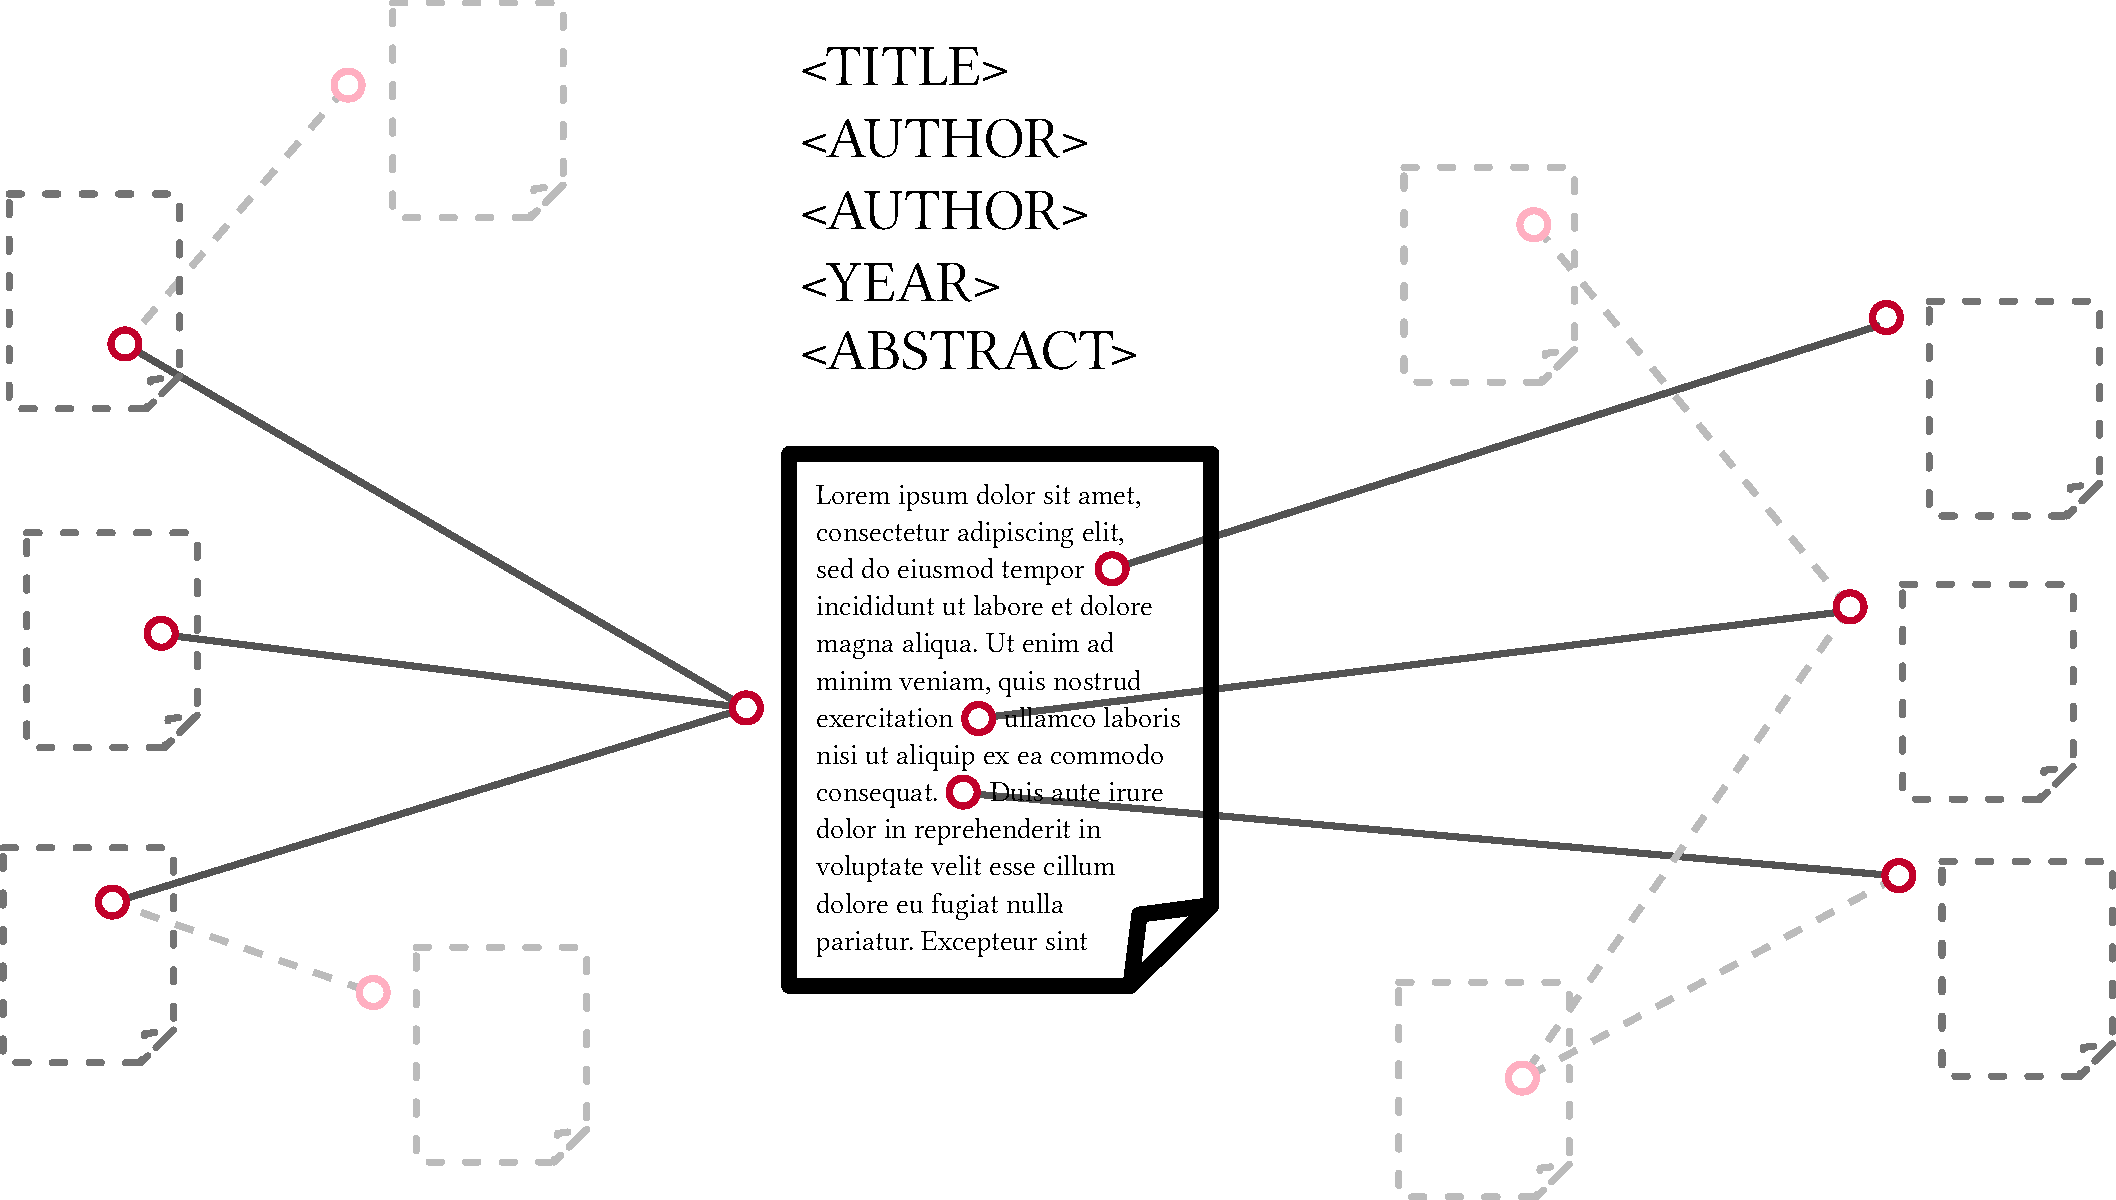
\includegraphics[width=0.8\textwidth]{figures/background/document_rich_view.pdf}
  \caption{Schematic view on a document, its metadata and embedding in the citation graph.}
  \label{fig:docrichview}
\end{figure}

\begin{figure}[t]
  \centering
    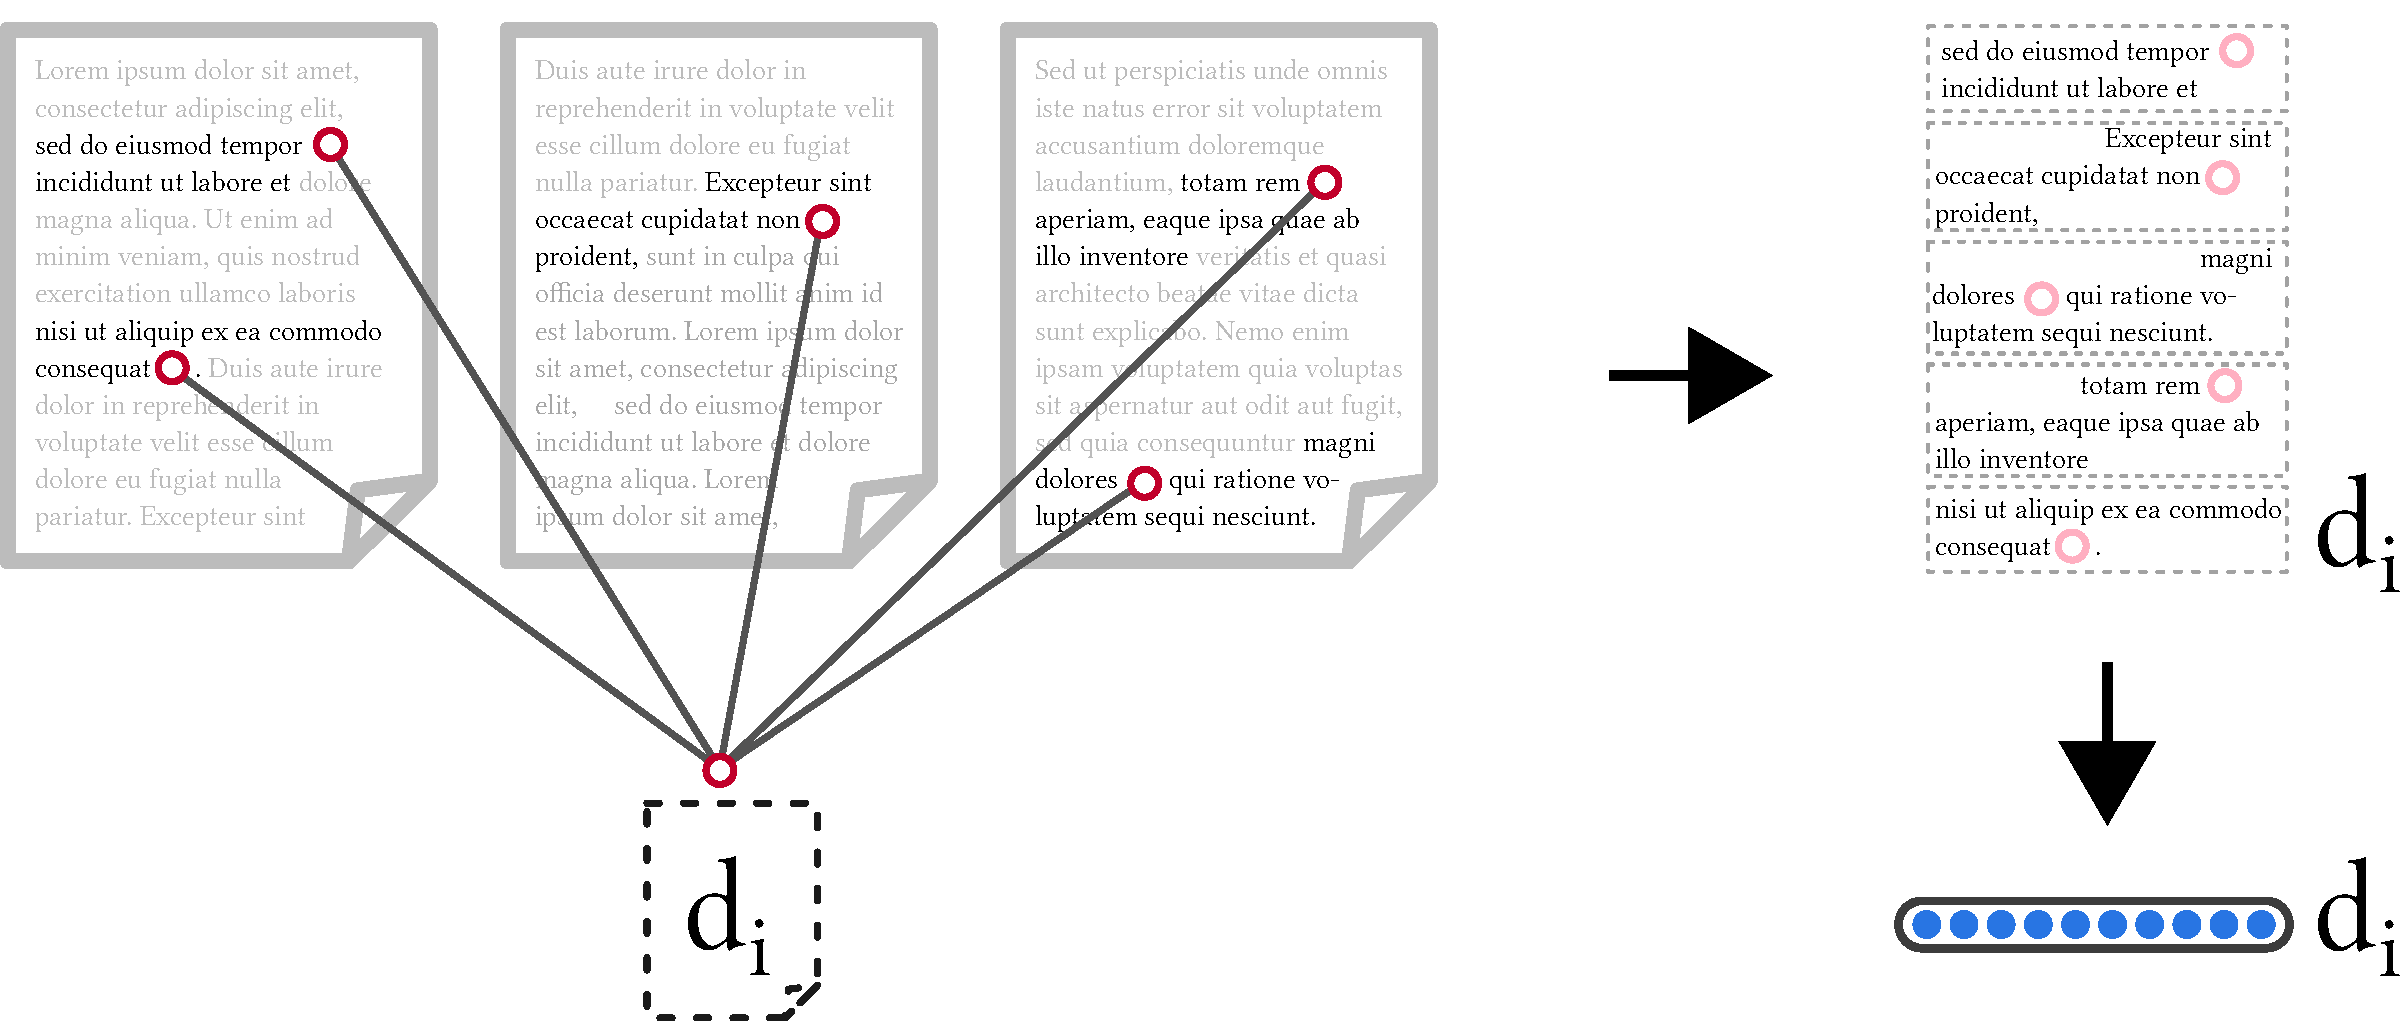
\includegraphics[width=\textwidth]{figures/background/document_context_view_withvec.pdf}
  \caption{Schematic visualization of a document's representation using citation contexts.}
  \label{fig:doccontview}
\end{figure}

As mentioned above, the focus in the case of citation recommendation lies on the candidate items---which are scientific publications. Figure~\ref{fig:docrichview} shows the types of information that are available to describe them. First and foremost each publication has, of course, its textual contents. Alongside this it is also part of a network of citations, meaning is has documents it is being cited by as well as documents it is citing. Lastly, there may also be metadata describing the document, such as the title, authors, year of publication etc. In order to study the viability of using explicit semantic representations of citation contexts for citation recommendation, without introducing any confounding variables, we will describe our documents \emph{only} by citation contexts. As citation contexts have been shown to contain information similar to and sometimes more extensive and focussed than abstracts~\cite{Elkiss2008}, we can expect decent recommendation results even though we're not taking any metadata associated with or textual content contained in the candidate documents into account. Figure~\ref{fig:doccontview} shows how a document representation can be generated from citation contexts. Document $d_i$ is cited by several other documents. By aggregating the contexts of these citations and deriving an abstract representation, $d_i$ can be represented by how it is being referenced in existing literature.
% Generating such representations of recommendation candidates is referred to as learning or training.

\begin{figure}[!b]
  \centering
    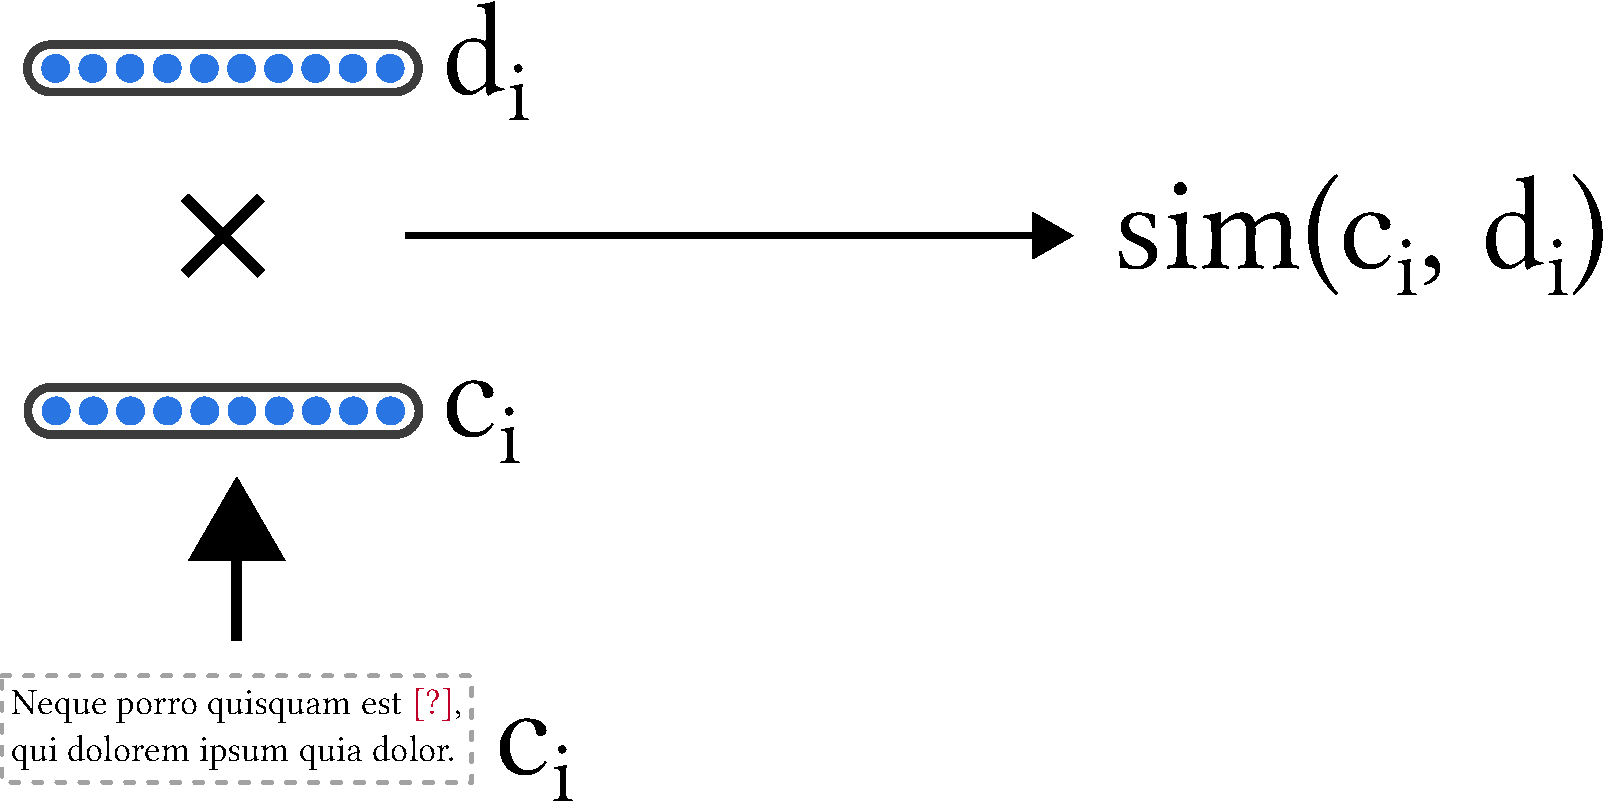
\includegraphics[width=0.7\textwidth]{figures/background/document_context_view_comparison.pdf}
  \caption{Schematic visualization of determining the similarity between an input citation contexts and a document representation.}
  \label{fig:doccomp}
\end{figure}

Recommendation itself is then done by taking a citation contexts $c_i$ as input, deriving an abstract representation in the same manner as was done for the aggregated contexts referencing a document, and then comparing the input's representation against those of all the documents. One such comparison is schematically depicted in Figure~\ref{fig:doccomp}. When every document---i.e., recommendation candidate---is associated with a similarity score, the system can output the most similar candidates as recommendations. With this, the overall picture looks as follows. The recommender system is trained on citation contexts, from which representations of the cited documents are learned. These documents are the publications the system is able to recommend. For a new context (without attached citation) given as input, the system identifies the documents most similar in the abstract representation space to the input and outputs these as recommendations.

\subsection{Evaluating citation recommendations}
Evaluation of recommender systems can be divided into three types, online evaluation, user study and offline evaluation. Online evaluation refers to monitoring naturally occurring user interaction with a system deployed online and drawing conclusions from metrics like click-through rates. User studies are conducted in a more controlled manner where users are aware of the evaluation and may be asked for explicit feedback on parts of the system. Offline evaluation differs from the other two types in that it does not directly involve human judgement. Rather, part of the data the system would, for online deployment, be trained on, is withheld and used as testing data. In doing this, past user judgement (like rating a movie or placing a citation) is used as a ground truth to test the system's output against. Because the human judgement is implicitly given within the data and can be processed automatically, offline evaluations can easily be performed on a large scale.~\cite{Aggarwal2016}

When recommending citations, abovementioned three types of evaluation can be realized as follows. Online evaluation can be performed by measuring which, if any, of the suggested publications a user actually inserts into their text. In a user study, participants can be asked to judge the relevance of recommended items while the system's input could be chosen by the user or given by the creators of the study. Lastly, offline evaluation as outlined above results in a re-prediction setting. That is, existing citation contexts are stripped of their citations, input into the system, and the resulting output compared to the original.

To aggregate relevance judgements of a large number of recommendations into a single number in order to compare different approaches, metrics are necessary. We use Recall, MRR, MAP and NDCG measured at different cut-off values. A cut-off, often denoted as \emph{Metric@}$k$, means only taking the top $k$ recommendations into consideration. This is done because, realistically, a user will not go through a list of hundreds of suggested items, but only look at the top three, five or maybe ten. Recall, MRR, MAP and NDCG with a cut-off $k$ can be defined as follows (see \cite{Aggarwal2016} for a more detailed, general discussion of these metrics):

Let $\mathcal{R} = r_1,r_2, ..., r_n$ be the ordered list of recommended items (highest to lowest) and ${\mathit{rel}(r_i)\in[0, 1]}$ denote the relevance of item $r_i$ at rank $i$. Furthermore let ${\mathcal{R}_{rel}=\{r_i|\mathit{rel}(r_i)=1\}}$ be the set of relevant items in an evaluation where $\mathit{rel}(r_i)\in\{0,1\}$---that is, an item is either relevant or not, with no partial relevance in between. Note that in a re-prediction setting as described above, $|\mathcal{R}_{rel}|=1$.

\paragraph{Recall} measures the fraction of the number of relevant items that was retrieved. If a cut-off $k$ is applied, the fraction's denominator is the minimum of the number of relevant items and the cut-off value.\[ \mathit{Recall}@k = \frac{\sum\limits_{i=1}^{k} \mathit{rel}(r_i)}{\mathit{min}(|\mathcal{R}_{rel}|,k)} \] For an evaluation with multiple test inputs, the mean over all Recall@k values is taken.

\paragraph{MRR} (mean reciprocal rank) is a metric often used when there is just one relevant item (e.g. re-prediction of a citation) or (when there are multiple relevant items) defined to just consider the first one. It takes into account the position of a recommended item through dividing its relevance by its rank.\[ \mathit{MRR}@k = \frac{\sum\limits_{i=1}^{k} \frac{\mathit{rel}(r_i)}{i}}{\mathit{min}(|\mathcal{R}_{rel}|,k)} \] Again, when evaluating over multiple test inputs, the mean over all MRR@k values is calculated.

\paragraph{MAP} (mean average precision) is the mean of average precision (\textbf{AP}) values of multiple queries. AP measures the average of all precision values at the ranks where relevant items are found. To define this, let $\rho(k)$ denote the number of relevant items within the first $k$ ranks. AP is then defined as \[ \mathit{AP}@k = \frac{\sum\limits_{i=1}^{k} \frac{\rho(i)}{i}\times\mathit{rel}(r_i)}{\mathit{max}(\rho(k), 1)} \] where $\mathit{rel}(r_i)\in\{0,1\}$. The value of MAP@k is the mean AP@k over all evaluated queries.

\paragraph{NDCG} (normalised discounted cumulative gain) is a metric compatible with non-binary relevance values that, similar to MAP, places higher weight on top ranks. It is calculated as the DCG (discounted cumulative gain) over the IDCG (ideal discounted cumulative gain)
 \[ \mathit{NDCG}@k = \frac{DCG@k}{IDCG@k} \]
where DCG is a sum of discounted relevance values
 \[ \mathit{DCG}@k = \sum\limits_{i=1}^{k} \frac{2^{\mathit{rel}(r_i)}-1}{\mathit{log}_2(i+1)} \]
and IDCG is a normalization factor to get values between zero and one, derived from an ideal recommendation $\mathcal{R}_{\mathit{ideal}}$ in which all items are ordered from the most relevant to the least
 \[ \mathit{IDCG}@k = \sum\limits_{r\in\mathcal{R}_{\mathit{ideal}}}\frac{2^{\mathit{rel}(r)}-1}{\mathit{log}_2(i+1)} \]
Likewise to the other metrics, the mean is calculated when evaluating over a set of test inputs.

    \chapter{Approach}\label{chap:approach}
approach approach.

\section{Problem Definition}
define define.

    \chapter{Experiments}\label{chap:experiments}
experiment experiment

\begin{table}[ht]
\begin{center}
    % \caption{Overview of existing data sets.}
    % \label{tab:existing-data-sets}
    \begin{tabular}{llllll}
    \toprule
    Data set & \#Papers & Cit. context & Disciplines & Full text & Ref. IDs \\
    \midrule
    arXiv CS    &  90K & 1 sentence & CS & yes & DBLP \\ % \cite{Faerber2018LREC}
    CiteSeerX /RefSeer  &  1M & 400 chars & all & no & no \\ % \cite{Caragea2014} / \cite{HuangWCMG15}
    PubMed Central OA\footnote{\url{https://www.ncbi.nlm.nih.gov/pmc/tools/openftlist/}} & 2.3M & extractable & Biomed./Life Sci. & yes & mixed \\
    Scholarly v2\footnote{\url{http://www.comp.nus.edu.sg/~sugiyama/SchPaperRecData.html}}  & 100K & extractable & CS & yes & no \\
    ACL-ARC  & 11k & extractable & CS/comp. ling. & yes & no \\ % \cite{Bird2008ACLARC}
    ACL-AAN  & 18k & extractable & CS/comp. ling. & yes & no  \\ % \cite{Radev2013}
    \bottomrule
    \end{tabular}
\end{center}
    \caption[Table caption]{\textbf{Table caption.} foo bar...\\}
    \label{tab:accuracy}
\end{table}


    \chapter{Conclusion}\label{chap:conclusion}
conclude conclude.

    \chapter{Acknowledgments}
acknowledge acknowledge.

\begin{itemize}
\item{advisers}
\item{examiner}
\item{person1 for the x}
\item{person2 for the y}
\end{itemize}


    % bibliography is not in the table of contents per default, add it manually
    % enable the \renewcommand for german header
    % \renewcommand{\bibname}{Literaturverzeichnis}
    \addcontentsline{toc}{chapter}{Bibliography}

    \bibliographystyle{ieeetr}
    \bibliography{bib/paper}
    \newpage
    \thispagestyle{empty}
    \mbox{}


\end{document}
